\chapter{Introducción}
\label{chap1}
\chapterquote
%~ {Don't get involved in partial problems, 
%~ but always take flight to where there is a free view over the whole single great problem, 
%~ even if this view is still not a clear one.}
{No se involucre en problemas parciales,
siempre tome vuelo hacia donde hay una vista libre sobre el gran problema único,
incluso cuando esta visión todavía no sea clara.}
{Ludwig Wittgenstein, 1889-1951}

\section{Motivación}
\label{1:motivacion}

La creciente sofisticación en los análisis de ingeniería demanda el estudio de sistemas cada vez más complejos.
Un ejemplo actual de esto es el modelado de grandes componentes termohidráulicos de geometría muy compleja en la industria nuclear. 
Es notable la presencia de subsistemas de caracterísiticas muy diferentes: principalmente diferentes tamaños y regímenes de flujos. 
Si bien se necesita modelar y entender el sistema completo, solo es de interés el detalle en algunos subsistemas. 
Algunos, como las tuberías, se hallan muy bien caracterizados por modelos simple (ODE's).
Otros, en cambio, requieren un análisis detallado de flujo, y por ello es necesaria la simulación fluidodinámica computacional (CFD).

En este marco se justifica el desarrollo de una técnica numérica que permita desglosar el problema general 
para analizar cada subsistema por separado mediante condiciones de borde dinámicas.
Como referencia a este enfoque se citan los trabajos desarrollados por J. S. Leiva y G. C. Buscaglia (2006) \cite{coup-0d3d}, P.J. Blanco et al. (2010) \cite{coup-black} y J. S. Leiva et al. (2011) \cite{coup-hyd}.

\section{Abordaje del modelado}
\label{1:abordaje}

\subsection{Desglosado del sistema original en subsistemas acoplados}
\label{1:acoplamiento}

Dado un sistema $S$ en un dominio $\Omega$ con borde $\Gamma$, es posible desglosar este dominio en $N$ particiones 
y analizar diferentes subsistemas $S_i,i=1,...,N$ por separado, acoplados entre sí mediante condiciones de borde en las uniones
(método de descomposición disjunta de dominios \cite{ddmethod}).
Las condiciones de borde originales del problema, impuestas sobre la curva $\Gamma$,
ahora se imponen sobre cada fragmento de la curva.
La Figura \ref{esquema-acoplamiento} presenta el esquema propuesto.
La notación utilizada es la siguiente:
\begin{itemize}
\item $S_i$ representa al subsistema $i$, $i=1,...,N$.
\item $U_{i,j}^k$ es la unión $k$ entre subsistemas $i$ y $j$, $k=1,...,K_{i,j}$.
\item $I_{S_i}^{l}$ es la interfaz local $l$ del subsistema $i$, $l=1,...,L_i$.
\item $\Gamma_i$ es la porción de frontera exterior en el subsistema $N$,
 $\Gamma_1$ $\cup$ $\Gamma_2$ $\cup$ ... $\cup$ $\Gamma_i$ ...  $\cup$ $\Gamma_N$ = $\Gamma$.
 Notar que $\Gamma_j$ puede ser nula para algún $S_j$.
\item ${(x_m)_{S_i}^{I_l}}$ es el valor de la variable $x_m$ en la interfaz ${l}$ del subsistema ${i}$, $m=1,...,M_i$.
\item ${(\bar{x})_{S_i}^{I_l}}$ es el vector de incógnitas $\{x_1,x_2,...,x_{M_i}\}$ en la interfaz ${l}$ del subsistema ${i}$.
\end{itemize}

\begin{figure}[ht]
\centering{}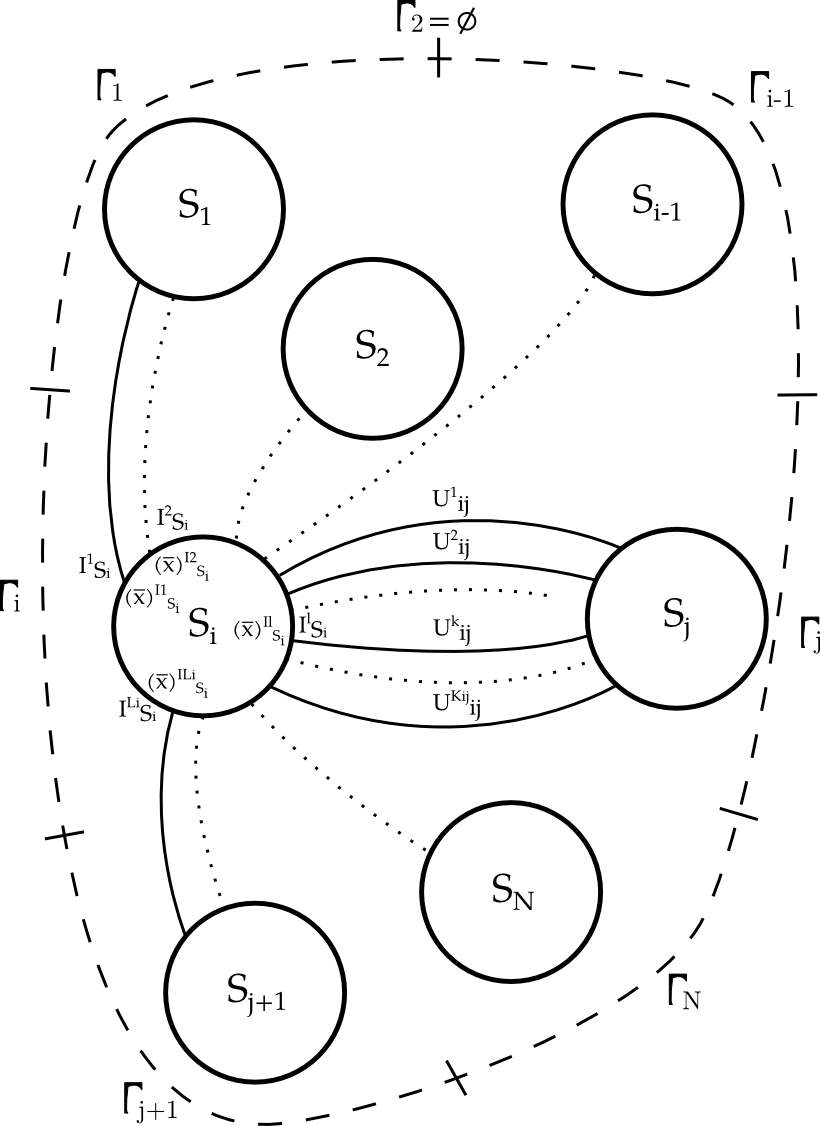
\includegraphics[scale = 0.4]{coupling_systems.png}
\caption[Esquema de descomposición disjunta de dominios]{Esquema de subsistemas de estudio relacionados mediante condiciones de borde dinámicas en interfaces de acoplamiento.} 
\label{esquema-acoplamiento} 
\end{figure}

En principio, existen tantas incógnitas como valores de variables en cada interfaz.
Sin embargo, es posible notar que la unión $U_{i,j}^k$ que relaciona los sistemas $S_{i}$ y $S_{j}$ 
mediante las interfaces $I_{S_{i}}^{l_1}$ e $I_{S_{j}}^{l_2}$ respectivamente, 
define una relación de continuidad
\footnote{
Las incógnitas que representan derivadas normales en la interfaz de acople pueden tomar signos opuestos según la convención.
Por ejemplo, si el flujo de calor es una incógnita, 
y se define como flujo positivo a aquel que es saliente del subsistema, 
entonces la condición de continuidad implicará que:
\begin{equation*}
{(q")_{S_i}^{I_{l_1}}}=-{(q")_{S_j}^{I_{l_2}}}
\label{continuidad-q}
\end{equation*}
}entre las incógnitas ${(x_m)_{S_i}^{I_{l_1}}}$ y ${(x_m)_{S_j}^{I_{l_2}}}$, de tal forma que:

\begin{equation}
{(x_m)_{S_i}^{I_{l_1}}}={(x_m)_{S_j}^{I_{l_2}}}
\label{continuidad}
\end{equation}
Estas relaciones reducen a la mitad la cantidad de incógnitas.
Las demás ecuaciones se encuentran a partir del modelo de estudio de cada subsistema. 
Sean $(F_m)_{i}^{l}$ las relaciones funcionales que calculan el valor de las incógnitas ${(x_m)_{S_i}^{I_l}}$ en la interfaz $l$ del subsistema $i$,
a partir del valor de otras incógnitas y de los datos de contorno sobre la frontera exterior $\Gamma_i$:

\begin{equation}
\begin{split}
  (x_m)_{S_i}^{I_l} = (F_m)_{i}^{l} \left ( (\bar{x})_{S_i}^{I_1}, (\bar{x})_{S_i}^{I_2}, ..., 
  (\bar{x})_{S_i}^{I_{L_i}}, (\alpha_i({\Gamma_i}) \right )
\end{split}
\label{ecuaciones-modelos}
\end{equation}
donde $(\alpha_i({\Gamma_i})$ representa las condiciones de borde impuestas sobre la curva $\Gamma_i$.
Notar que algunas de las dependencias pueden anularse dependiendo del modelo de estudio utilizado en cada subsistema
\footnote{
Cuando la expresión es más sencilla y solo involucra el valor de otro tipo de condición de borde en la misma interfaz,
la relación funcional recibe el nombre de operador \textit{Steklov-Poincaré}.
En matemática, el operador \textit{Steklov-Poincaré} mapea el valor de una condición de borde de una PDE elíptica en un dominio al valor
de otra condición de borde (por ejemplo, una condición de borde de tipo \textit{Dirichlet} en una condición de borde de tipo \textit{Neumann}).
Usualmente, cualquiera de las dos condiciones determinan la solución.
}.

\subsection{Sistema de ecuaciones a resolver}
\label{1:ecuaciones}
Restando el lado derecho en (\ref{ecuaciones-modelos}) a ambos lados, se obtienen relaciones del tipo:

\begin{equation}
(R_m)_{i}^{l} =   (x_m)_{S_i}^{I_l} - (F_m)_{i}^{l} \left ( (\bar{x})_{S_i}^{I_1}, (\bar{x})_{S_i}^{I_2}, ..., 
  (\bar{x})_{S_i}^{I_{L_i}}, (\alpha_i({\Gamma_i}) \right ) 
\label{ecuaciones-residuos}
\end{equation}
para cada residuo en la incógnita $m$ de cada interfaz $l$ del subsistema $i$.
Debido a las relaciones de continuidad (\ref{continuidad}), es posible descartar ecuaciones,
seleccionándolas de tal forma que el sistema de ecuaciones en cada subsistema quede bien planteado,
como se explica más adelante.
La convergencia fuerte de los subsistemas acoplados necesita que los residuos sean nulos.
El sistema global de ecuaciones restante se reduce a la siguiente expresión:

\begin{equation}
\bar{R}=\bar{0}
\label{sistema-simple}
\end{equation}
donde $\bar{R}$ es el vector de residuos de las ecuaciones seleccionadas.
En general estas relaciones son no lineales, y por lo tanto se resuelven de forma iterativa, a partir de un primer vector solución propuesto.
Debido a que en cada subsistema solo han sobrevivido ciertas relaciones funcionales, 
van a tomar como dato solo algunos de estos valores propuestos.
Es necesario por tanto seleccionar las ecuaciones de modo que el problema resulte bien planteado.
Por ejemplo, si interesara calcular el campo de temperaturas en un subsistema dado,
serían incógnitas la temperatura y el flujo de calor en cada una de sus interfaces.
Sin embargo ambas no pueden ser impuestas como dato en el mismo subsistema.
En general, cada subsistema debe recibir condiciones o bien de tipo \textit{Dirichlet}, o bien de tipo \textit{Neumann}, para cada ecuación.

\subsection{Métodos numéricos para la resolución de sistemas de ecuaciones de residuos}
\label{1:metodos}
Existen diferentes estrategias para hallar las raíces del sistema (\ref{sistema-simple}). 
La forma clásica es el conocido método \textit{Dirichlet-to-Neumann}, que resuelve mediante iteraciones de tipo \textit{Piccard}. La ventaja de este método es que es sencillo de implementar, ya que es un método explícito y por tanto, los valores calculados por algún subsistema son inmediatamente impuestos como condición de borde a otros subsistemas.
Sin embargo, tiene algunas desventajas.
Por ejemplo, las condiciones de borde que son datos en cada subsistema no pueden elegirse arbitrariamente. 
Las interfaces $I_{S_i}^{l_1}$ y $I_{S_j}^{l_2}$ comunes a cada unión $U_{i,j}^k$ 
deben alternar condiciones de borde de tipo \textit{Dirichlet} y de tipo \textit{Neumann} para las ecuaciones que relacionan las mismas variables de estado en cada subsistema.

El siguiente ejemplo esclarece lo expresado. Se desea resolver la ecuación de calor con condiciones de borde homogéneas, para encontrar el campo de temperaturas $u$ en una barra unidimensional de longitud $L$, fuente interna de energía $f$ y conductividad térmica $k$:

\begin{equation}
\left\{\begin{matrix}
-k \Delta u=f \\
\left.u\right|_{\partial\Omega}=0
\end{matrix}\right.
\end{equation}
mediante el método de descomposición disjunta de dominios (ver Figura \ref{temp-ej}. El dominio original $[0,L]$ es particionado en los subdominios $[0,c]$ y $[c,L]$.
\begin{figure}
\centering{}
\begin{tikzpicture}
	\node at (12.5,4em) (om) {$\Omega$};

	\node at (7.5,5.9em) (Olabel) {0}; % 0
	\node at (7.5,5em) (O) {}; % point 0

	\node at (14.5,6.9em) (clabel) {c}; % c
	\node at (14.5,5em) (c) {}; % point c

	\node at (17.5,5.9em) (llabel) {L}; % L
	\node at (17.5,5em) (l) {}; % point L

	\draw[line width=1pt, o-|] (O) -- (c.center); % primer extremo de barra completa
	\draw[line width=1pt, |-o] (c.center) -- (l); % segundo extremo de barra completa

	\draw[line width=0.8pt,->] (11,3.5em) -- (10,1.5em); % primer flecha
	\draw[line width=0.8pt,->] (16,3.5em) -- (17,1.5em); % segunda flecha

	\node at (10,-1em) (om1) {$\Omega_1$};
	\node at (6.5,0.9em) (O1label) {0};
	\node at (6.5,0em) (O1) {};
	\node at (13.5,0.9em) (c1label) {c};
	\node at (13.5,0em) (c1) {};

	\draw[line width=1pt, o-o] (O1) -- (c1); % primer barra

	\node at (17,-1em) (om2) {$\Omega_2$};
	\node at (15.5,0.9em) (c2label) {c};
	\node at (15.5,0em) (c2) {};
	\node at (18.5,0.9em) (l2label) {L};
	\node at (18.5,0em) (l2) {};

	\draw[line width=1pt, o-o] (c2) -- (l2); % segunda barra

\end{tikzpicture}
\caption[Descomposición en barra unidimensional]{Descomposición disjunta de dominios en el cálculo del campo de temperatura a lo largo de una barra unidimensional.}
\label{temp-ej}
\end{figure}
Para que cada problema quede bien planteado es necesario imponer una condición de borde extra en el punto de interfaz a cada lado.
En el método \textit{Dirichlet-to-Neumann}, es necesario decidir qué subsistema va a resolverse en primera instancia, a partir de algún valor supuesto en el borde.
Si arbitrariamente se decidiera imponer una temperatura (condición \textit{Dirichlet} al borde del primer subsistema,
luego de realizar el cálculo de temperaturas quedaría definido un flujo calórico a través de su interfaz de conexión con el segundo subsistema.
Este valor de flujo luego debe ser utilizado para imponerse como condición de borde al segundo subsistema,
en el cuál se resolverá el campo de temperaturas y quedará definida una nueva temperatura en la interfaz de acople.
Esta temperatura se impone nuevamente al primer subsistema, y el cálculo continúa así hasta que los sucesivos valores de las variables acopladas convergan.
Si inicialmente se hubiera impuesto una condición de \textit{Neumann} en el primer subdominio, necesariamente al segundo subdominio debe imponérsele una condición de \textit{Dirichlet}. Es decir, al utilizar el método \textit{Dirichlet-to-Neumann}, la elección de un tipo de frontera en un subdominio dado determina el tipo de frontera en el subdominio contiguo,
para las ecuaciones que relacionan las mismas variables de estado en ambos subsistemas.
Otra desventaja de este método es que en general requiere demasiadas iteraciones para converger \cite{fede-enief2016}. En algunos problemas el método puede quedar estancado, iterando en series de valores que se repiten en ciclo. Y en otros casos el método es divergente (sin ir más allá, para un cierto conjunto de parámetros del problema ejemplo analizado, el método diverge, ver \cite{coup-strong}).

Otra forma de resolver el problema es aplicando métodos para encontrar raíces a funciones vectoriales no lineales (sistema de ecuaciones de residuos \ref{sistema-simple} en función de las variables de acople incógnitas),
como por ejemplo, el método \textit{Newton-Raphson}.
Haciendo un desarrollo de Taylor de las ecuaciones de residuos alrededor del punto $\bar{x}_n$, truncando los términos superiores al primer orden, y evaluando en $x=x_{n+1}$ se tiene:

\begin{equation}
\bar{R}(\bar{x}) = \bar{R}(\bar{x}_n) + \nabla \bar{R}(\bar{x}_n)(\bar{x}_{n+1}-\bar{x}_n)
\label{taylor}
\end{equation}
donde $\nabla \bar{R}(\bar{x}_n)$ es la matriz jacobiana del sistema $J$ evaluada en el punto $\bar{x}_n$, donde el elemento $J_{ij}$ debe evaluarse como $J_{ij}=\frac{\partial R_i}{\partial x_j}$.
Suponiendo que ${x_{n+1}}$ tiende a la raíz buscada se ha de cumplir que $\bar{R}(\bar{x}_{n+1})=0$. Sustituyendo en \ref{taylor} y operando algebraicamente se llega a la siguiente expresión:

\begin{equation}
\bar{R}(\bar{x}_n) = -J(\bar{x}_n)(\bar{x}_{n+1}-\bar{x}_n)
\end{equation}
que es el método de iterativo $Newton-Raphson$ con orden de convergencia cuadrática. Para hallar la solución $\bar{x}_{n+1}$ simplemente hay que resolver el sistema:

\begin{equation}
\bar{x}_{n+1} = \bar{x}_{n} -J^{-1}(\bar{x}_n)\bar{R}(\bar{x}_n)
\end{equation}
El problema es que para utilizar este método se requiere la construcción de la matriz jacobiana en cada iteración, lo cual es demasiado costoso.
Una sencilla aproximación mediante diferencias finitas de primer orden de cada elemento de la matriz jacobiana requiere numerosas ejecuciones de códigos clientes
\footnote{
Cada elemento $J_{ij}=\frac{\partial R_i}{\partial x_j}$ puede aproximarse mediante diferencias finitas a primer orden como:
\begin{equation}
J_{ij} \approx \frac{R_i(x_j + \Delta x_j) - R_i(x_j)}{\Delta x_j}
\end{equation}
La construcción de la matriz jacobiana con éste método requiere una evaluación del vector residuo $\bar{R}$ en el punto $\bar{x}$ y luego $N$ evaluaciones extras, donde $N$ es la cantidad de incógnitas. Es decir, en total, se requieren $N+1$ ejecuciones de cada código cliente.
}.
Si bien estas evaluaciones son independientes entre sí y por lo tanto altamente paralelizables, este método es excesivamente costoso.

Una forma alternativa y elegante de resolver el sistema de ecuaciones planteado en \ref{sistema-simple} es mediante métodos \textit{quasi-Newton}.
Estos métodos tienen convergencia superlineal \cite{broyden-on}, y por lo tanto presentan una ventaja frente a los métodos mediante iteraciones de \textit{Piccard}. 
La característica principal de estos métodos es que aproximan la matriz jacobiana sin necesidad de realizar evaluaciones extras, y por lo tanto tienen también un punto de ventaja frente al método de \textit{Newton-Raphson}.
El método de \textit{Broyden} es uno de ellos \cite{broyden}.
También existe otra variante del método, el método \textit{Broyden ortonormal}, que asegura la convergencia en $N$ iteraciones para sistemas lineales \cite{broyden-on}, donde $N$ es la dimensión de la matriz jacobiana.

Existe también un conjunto de métodos conocidos como métodos \textit{Newton-Krylov} para la resolución del sistema \ref{sistema-simple}. Estos métodos no requieren el cálculo de matriz jacobiana ya que resuelven el sistema mediante gradientes descendientes, gradientes conjugados y otras técnicas que también serán exploradas en el presente trabajo. Sin embargo, en cada paso de descenso requieren evaluaciones de residuos, y por tanto son altamente costosos.

\subsection{Problemas de evolución temporal}
\label{1:evolucion}
En problemas de avance temporal la estrategia de selección de variables que son datos o incógnitas en cada interfaz puede variar en la evolución.
Cabe resaltar también que no existe necesidad de que los cálculos en cada subsistema utilicen el mismo paso temporal.
Cualquiera de los códigos podría utilizar subdivisiones del paso temporal del otro código,
y establecer el acople sólo en pasos de tiempo determinados.
Los valores para las condiciones de borde dinámicas entre los pasos de tiempo en los que efectivamente se intercambian datos,
pueden interpolarse con valores previos.

Notar que la herramienta es incondicionalmente estable debido a que 
en cada paso de tiempo se asegura la convergencia fuerte de los valores de las variables en las interfaces de acople.

\section{Objetivos y estructura de trabajo}
\label{1:objetivos}
Considerando la motivación y la formulación precedente, queda establecido el siguiente objetivo general de la maestría:

\vspace{1em}
\begin{addmargin}[1.5em]{1.5em}
\textit{Implementar el acoplamiento fuerte entre modelos dimensionalmente heterogéneos,
resolviendo cada subdominio por separado con códigos particulares, e imponiendo la
interacción entre ellos sólo mediante condiciones de borde.}
\end{addmargin}
\vspace{1em}

La estructura de la tesis es detallada a continuación.
En el presente \hyperlink{chapter.1}{capítulo} se han planteado las ecuaciones que surgen al dividir sistemas complejos mediante interfaces con condiciones de borde dinámicas,
y se han presentado alternativas numéricas para la resolución de las mismas.
En el \hyperlink{chapter.2}{Capítulo 2} se describen las diferentes formas de implementar el acoplamiento entre códigos que han sido investigadas e implementadas,
se presenta la estructura de comunicación definida y se describe la arquitectura de acoplamiento necesaria a ser implementada en los códigos comunicados por paso de mensajes.
En el \hyperlink{chapter.3}{Capítulo 3} se muestran algunas aplicaciones de la herramienta estudiada,
presentando distintos códigos utilizados para realizar cálculos fluidodinámicos.
La primera aplicación es un sistema fluídico cerrado que se estudia subdividiéndolo en dos subsistemas, con dos interfaces de acople cada uno.
El movimiento del fluido está gobernado por fuerzas naturales y por lo tanto interesa acoplar variables de 
caudal, presión, temperatura y flujo de calor en cada interfaz.
El siguiente sistema de estudio es el vaciado del tanque reflector del reactor de investigación RA-10.
Interesa analizar los tiempos de descarga ya que el mismo es diseñado como Segundo Sistema de Parada (SSP).
Se abordan distintos modelos multiescala del mismo, para estudiar el detalle fluídico tridimensional en un componente del sistema,
acoplando con condiciones de borde dinámicas a modelos cero-dimensionales que representan el resto del sistema.
Al final del capítulo se presenta un estudio de redes hidráulicas con múltiples componentes,
para demostrar la eficiencia de la herramienta en acoples de mayor escala.
En éstos últimos ejemplos comentados, las variables incógnitas en las interfaces de acoplamiento son velocidades (o caudales) y fuerzas (presiones y tensiones de corte).
En el \hyperlink{chapter.4}{Capítulo 4} se extiende la técnica de acople a problemas que involucran otros modelos físicos.
Se describe el código maestro de acople multifísico desarrollado y se presentan ejemplos de aplicación en el problema neutrónico-termohidráulico.

